% ============================================================
%  Fundamentos económicos para el análisis cuantitativo de la gestión
%  Material teórico del Laboratorio de Métodos Cuantitativos (FCE-UBA)
%  Autores: Manuel  ·  Juan Ignacio da Torre
%  Compilar con: pdflatex main.tex  (x2 para el índice/refs)
% ============================================================
\documentclass[11pt,a4paper,oneside]{report}

% --- Idioma y codificación ---
\usepackage[utf8]{inputenc}
\usepackage[T1]{fontenc}
\usepackage[spanish,es-noshorthands]{babel} % es-noshorthands evita el punto decimal activo de babel-spanish
\usepackage{lmodern}
\usepackage{microtype}

% --- Matemática ---
\usepackage{amsmath,amssymb,amsthm,mathtools}

% --- Tablas y figuras ---
\usepackage{graphicx}
\usepackage{booktabs}
\usepackage{array}
\usepackage{multirow}
\usepackage{caption}

% --- Diseño ---
\usepackage[a4paper,margin=2.6cm]{geometry}
\usepackage{xcolor}
\definecolor{azulcat}{RGB}{20,70,130}
\definecolor{grissuave}{RGB}{90,90,90}
\usepackage[most]{tcolorbox}
\usepackage{enumitem}
\setlist{itemsep=2pt,topsep=3pt}
\usepackage{fancyhdr}
\usepackage{titlesec}

% --- Hipervínculos ---
\usepackage[colorlinks=true,linkcolor=azulcat,citecolor=azulcat,urlcolor=azulcat]{hyperref}

% --- Encabezados ---
\pagestyle{fancy}
\fancyhf{}
\fancyhead[L]{\small\itshape Fundamentos económicos para la gestión}
\fancyhead[R]{\small\thepage}
\renewcommand{\headrulewidth}{0.4pt}

% --- Entornos tipo teorema ---
\theoremstyle{definition}
\newtheorem{definicion}{Definición}[chapter]
\newtheorem{ejemplo}{Ejemplo}[chapter]
\newtheorem{propiedad}{Propiedad}[chapter]

% --- Caja "puente al laboratorio" ---
\newtcolorbox{labbox}[1][Del concepto al código]{
  colback=azulcat!4, colframe=azulcat, fonttitle=\bfseries,
  coltitle=white, title=#1, breakable, boxrule=0.6pt, arc=2pt,
  left=6pt,right=6pt,top=4pt,bottom=4pt}

% --- Caja "idea clave" ---
\newtcolorbox{ideabox}{
  colback=orange!6, colframe=orange!70!black, boxrule=0.6pt, arc=2pt,
  left=6pt,right=6pt,top=4pt,bottom=4pt}

% --- Macros económicas ---
\newcommand{\van}{\mathrm{VAN}}
\newcommand{\tir}{\mathrm{TIR}}
\newcommand{\img}{I_{\mathrm{mg}}}
\newcommand{\cmg}{C_{\mathrm{mg}}}
\newcommand{\cme}{C_{\mathrm{me}}}
\newcommand{\dd}{\,\mathrm{d}}

\titleformat{\chapter}[display]
  {\normalfont\huge\bfseries\color{azulcat}}{\chaptertitlename\ \thechapter}{12pt}{\Huge}

% ============================================================
\begin{document}

% ---------- PORTADA ----------
\begin{titlepage}
\centering
\vspace*{1.2cm}
{\scshape\large Universidad de Buenos Aires\\ Facultad de Ciencias Económicas\par}
\vspace{0.4cm}
{\scshape Laboratorio de Métodos Cuantitativos Aplicados a la Gestión\par}
\vspace{1.8cm}
{\color{azulcat}\rule{\linewidth}{1.2pt}\par}
\vspace{0.8cm}
{\Huge\bfseries Fundamentos económicos para el análisis cuantitativo de la gestión\par}
\vspace{0.6cm}
{\large\itshape Una introducción aplicada, de la teoría a la computación\par}
\vspace{0.6cm}
{\color{azulcat}\rule{\linewidth}{1.2pt}\par}
\vspace{2.2cm}
{\large\bfseries Manuel \quad\textbullet\quad Juan Ignacio da Torre\par}
\vspace{0.3cm}
{\small\color{grissuave} Cátedra de Métodos Cuantitativos Aplicados a la Gestión\par}
\vfill
{\large Material teórico de cátedra\par}
\vspace{0.3cm}
{\large Junio de 2026\par}
\end{titlepage}

% ---------- RESUMEN ----------
\thispagestyle{plain}
\chapter*{Resumen}
\addcontentsline{toc}{chapter}{Resumen}

Este documento reúne, en un solo lugar, los \textbf{fundamentos económicos} que sostienen las prácticas computacionales del Laboratorio de Métodos Cuantitativos Aplicados a la Gestión. Su objetivo es que cada herramienta que usás en las \emph{notebooks} —graficar una función de costos, resolver un equilibrio de mercado, derivar para hallar un beneficio máximo, integrar para medir un excedente o descontar un flujo de fondos— tenga detrás una \textbf{teoría clara, explicada desde cero y conectada con los grandes autores de la disciplina}.

No es un libro de programación: acá no hay código. Es el \emph{por qué} económico que va antes del \emph{cómo} computacional. Asumimos que recién te estás acercando tanto a la economía como a Python, de modo que cada concepto se construye paso a paso, con definiciones, intuición, un ejemplo numérico resuelto y una caja final —\textsf{Del concepto al código}— que anticipa cómo ese mismo concepto reaparece en el laboratorio.

A lo largo del texto dialogamos con la forma en que estos temas son presentados por referentes como Varian~\cite{varian}, Pindyck y Rubinfeld~\cite{pindyck}, Mankiw~\cite{mankiw}, Stiglitz~\cite{stiglitz}, Blanchard~\cite{blanchard} y Chiang~\cite{chiang}, entre otros, buscando una síntesis honesta y accesible más que una exposición enciclopédica.

\bigskip
\noindent\textit{Palabras clave:} microeconomía aplicada, análisis marginal, optimización, evaluación de inversiones, métodos cuantitativos, economía computacional.

\vspace{1cm}
% ---------- ÍNDICE ----------
\tableofcontents
\thispagestyle{plain}

% ============================================================
%  CUERPO
% ============================================================
\chapter{Prefacio: por qué la economía necesita números}
\label{cap:prefacio}

\section{La gestión es decidir con información}

Gestionar una organización —una empresa, una cooperativa, un hospital, un Estado— es, en el fondo, \textbf{tomar decisiones bajo escasez}. Hay un presupuesto limitado, una capacidad de producción limitada, un tiempo limitado y una demanda que reacciona a lo que hacemos. La economía es precisamente la disciplina que estudia cómo se asignan recursos escasos entre fines alternativos, y por eso ofrece un marco natural para pensar la gestión.

Ahora bien, durante mucho tiempo esas decisiones se tomaron «a ojo», apoyadas en la experiencia. El cambio de las últimas décadas es que hoy disponemos de \textbf{datos} y de \textbf{herramientas de cálculo} que permiten cuantificar lo que antes era intuición. Saber que «si subo el precio, vendo menos» es economía básica; saber \emph{cuánto} menos vendo, a partir de los datos de mi propio negocio, es economía cuantitativa aplicada. Esa diferencia —pasar del signo a la magnitud— es el corazón de este curso.

\begin{ideabox}
\textbf{Idea central del Laboratorio.} La teoría económica nos dice \emph{qué} relación esperar entre variables (precio y cantidad, costo y producción, inversión y rentabilidad); las herramientas computacionales nos dicen \emph{cuánto} vale esa relación con los datos concretos que tenemos enfrente. Una sin la otra queda coja.
\end{ideabox}

\section{Qué vas a encontrar en este material}

Este texto recorre, en orden, los bloques económicos del Laboratorio:

\begin{enumerate}
  \item \textbf{Datos, variables y visualización} (Capítulo~\ref{cap:datos}): el punto de partida práctico.
  \item \textbf{Funciones económicas} (Capítulo~\ref{cap:funciones}): demanda, oferta, costos, ingreso y beneficio.
  \item \textbf{Equilibrio de mercado y sistemas de ecuaciones} (Capítulo~\ref{cap:equilibrio}).
  \item \textbf{El modelo insumo-producto de Leontief} (Capítulo~\ref{cap:leontief}).
  \item \textbf{Análisis marginal y derivadas} (Capítulo~\ref{cap:marginal}).
  \item \textbf{Elasticidades} (Capítulo~\ref{cap:elasticidad}).
  \item \textbf{Integrales y excedentes} (Capítulo~\ref{cap:integrales}).
  \item \textbf{Optimización económica} (Capítulo~\ref{cap:optimizacion}).
  \item \textbf{Competencia imperfecta: el duopolio} (Capítulo~\ref{cap:duopolio}).
  \item \textbf{Evaluación de proyectos de inversión} (Capítulo~\ref{cap:inversiones}).
\end{enumerate}

Cada capítulo sigue la misma estructura pensada para quien recién arranca: primero la \emph{intuición} (qué problema de gestión resolvemos), después la \emph{definición formal} y las fórmulas, luego un \emph{ejemplo numérico} resuelto a mano, y al final una caja \textsf{Del concepto al código} que muestra cómo ese mismo concepto reaparece —ya como herramienta— en las \emph{notebooks} de Python del laboratorio.

\section{Una aclaración sobre los prerrequisitos}

Esta materia combina dos mundos: la \textbf{economía} y la \textbf{programación}. Es posible que vengas con base en uno y no en el otro, o en ninguno. Por eso el material parte de cero en lo económico: no damos por sabido qué es una función de demanda ni qué significa «maximizar el beneficio». Si algún concepto te resulta nuevo, es esperable; está explicado dentro del propio texto y referenciado a manuales clásicos por si querés profundizar.

Lo que sí conviene tener fresco son tres herramientas matemáticas que usaremos como lenguaje: las \emph{funciones} (cómo una variable depende de otra), las \emph{derivadas} (cómo medir un cambio) y las \emph{integrales} (cómo acumular). Las tres se repasan en los capítulos donde hacen falta, siguiendo el enfoque de Chiang y Wainwright~\cite{chiang} y de Sydsæter y Hammond~\cite{sydsaeter}, pensados justamente para economistas que no son matemáticos profesionales.

\section{Cómo leer las fórmulas sin asustarse}

Una fórmula económica es una frase escrita en taquigrafía. Cuando veas, por ejemplo,
\[
\Pi(q) = I(q) - C(q),
\]
leelo en castellano: «el beneficio $\Pi$ que obtengo al producir una cantidad $q$ es igual al ingreso $I$ que genera esa cantidad, menos el costo $C$ de producirla». Toda la matemática del curso es de este tipo: traducciones precisas de ideas económicas razonables. Si entendés la idea, la fórmula deja de dar miedo.

Con esa actitud —entender antes que memorizar— arrancamos.

\chapter{Datos, variables y visualización}
\label{cap:datos}

\section{Antes de la teoría: los datos}

La economía cuantitativa de la gestión arranca, en la práctica, con un archivo de datos: una planilla de ventas, un registro de afiliados, un histórico de precios. Antes de modelar nada, hay que entender qué tenemos entre manos. Este capítulo presenta el vocabulario mínimo del análisis de datos —qué es una variable, de qué tipo, cómo resumirla y cómo mostrarla— que después usaremos para alimentar todos los modelos económicos del libro. Fue, además, uno de los temas que los estudiantes más valoraron del curso, porque es el más cercano al trabajo real con datos.

\section{La estructura de un conjunto de datos}

Un \textbf{conjunto de datos} (o \emph{dataset}) se organiza como una tabla:
\begin{itemize}
  \item Cada \textbf{fila} es una \emph{observación} o unidad de análisis (un cliente, un día, una sucursal, un producto).
  \item Cada \textbf{columna} es una \emph{variable}: una característica medida de esas observaciones (precio, cantidad, región, fecha).
\end{itemize}
Esta forma «ordenada» —una observación por fila, una variable por columna— es la que permite calcular, agrupar y graficar con comodidad.

\section{Tipos de variables}

Saber con qué tipo de variable trabajamos determina qué cálculos y qué gráficos tienen sentido. La distinción básica es:

\begin{center}
\renewcommand{\arraystretch}{1.3}
\begin{tabular}{p{3.2cm} p{4.0cm} p{5.0cm}}
\toprule
\textbf{Tipo} & \textbf{Subtipo} & \textbf{Ejemplo} \\
\midrule
\multirow{2}{*}{\textbf{Cuantitativa}} & Continua (mide) & precio, peso, ingreso \\
 & Discreta (cuenta) & cantidad de unidades, n.\textsuperscript{o} de clientes \\
\midrule
\multirow{2}{*}{\textbf{Cualitativa}} & Nominal (sin orden) & región, rubro, color \\
 & Ordinal (con orden) & nivel de satisfacción (1 a 5), categoría A/B/C \\
\bottomrule
\end{tabular}
\end{center}

Con una variable \emph{cuantitativa} tiene sentido calcular un promedio; con una \emph{cualitativa nominal}, no (el «promedio» de las regiones no significa nada), pero sí contar frecuencias. Confundir estos tipos es uno de los errores más comunes al empezar.

\section{Calidad de los datos: faltantes y limpieza}

Los datos reales vienen «sucios»: valores faltantes, errores de carga, duplicados. Antes de analizar hay que \textbf{limpiar}. El problema más frecuente son los \emph{valores faltantes} (celdas vacías). Hay dos caminos: descartar las filas afectadas (si son pocas) o \textbf{imputar} un valor razonable.

\begin{ideabox}
\textbf{Regla práctica útil.} Para imputar una variable \emph{ordinal} en escala (por ejemplo, una encuesta de satisfacción de 1 a 5), conviene usar la \textbf{mediana} antes que la media: es robusta a valores extremos y no devuelve un número fuera de la escala (un 3, no un 3{,}47). Para variables continuas, la media suele ser adecuada si no hay valores atípicos marcados.
\end{ideabox}

\section{Medidas de resumen}

Para describir una variable cuantitativa con pocos números usamos:
\begin{itemize}
  \item \textbf{Tendencia central:} la \emph{media} (promedio) y la \emph{mediana} (el valor del medio). Cuando difieren mucho, hay asimetría o valores extremos.
  \item \textbf{Dispersión:} el \emph{desvío estándar} mide cuánto se alejan los datos de la media; el \emph{rango} y los \emph{cuartiles} describen cómo se reparten.
\end{itemize}
La mediana y los cuartiles son más \emph{robustos} que la media: un solo valor disparatado (un precio cargado con un cero de más) arrastra a la media pero casi no mueve a la mediana. En gestión, donde los errores de carga son comunes, esa robustez importa.

\section{Visualización: mostrar para entender}

Un gráfico bien elegido comunica en un vistazo lo que una tabla esconde. Los parciales del curso suelen pedir «al menos tres gráficos de distinta naturaleza», justamente para practicar esta elección. Los cuatro básicos:

\begin{center}
\renewcommand{\arraystretch}{1.3}
\begin{tabular}{p{3.4cm} p{4.2cm} p{4.8cm}}
\toprule
\textbf{Gráfico} & \textbf{Sirve para} & \textbf{Variable(s)} \\
\midrule
Histograma & ver la \emph{distribución} de una variable & 1 cuantitativa \\
Boxplot (caja) & ver mediana, dispersión y \emph{atípicos} & 1 cuantitativa (por grupos) \\
Barras & comparar \emph{categorías} & 1 cualitativa + 1 medida \\
Dispersión (scatter) & ver la \emph{relación} entre dos variables & 2 cuantitativas \\
\bottomrule
\end{tabular}
\end{center}

La regla de oro: \textbf{el tipo de variable manda sobre el tipo de gráfico}. Una variable cuantitativa pide histograma o boxplot; una cualitativa, barras; una relación entre dos cuantitativas, un diagrama de dispersión (que, no por casualidad, es el primer paso para intuir las funciones de demanda y costo de los próximos capítulos). Todo gráfico debe llevar título y ejes rotulados: sin eso, no comunica.

\begin{labbox}
Este capítulo es el reino de \texttt{pandas} y \texttt{matplotlib}. Con \texttt{pandas} se carga la tabla (\texttt{read\_csv}), se la inspecciona (\texttt{info()}, \texttt{describe()}), se cuentan faltantes (\texttt{isna().sum()}), se imputan (\texttt{fillna(...)}) y se agrupan categorías (\texttt{groupby(...).mean()}). Con \texttt{matplotlib} se construyen los cuatro gráficos de la tabla anterior. Es el bloque más práctico del curso y la puerta de entrada a todo lo demás: sin datos limpios y bien entendidos, los modelos económicos no se sostienen.
\end{labbox}

\section{Síntesis del capítulo}

Antes de modelar hay que conocer los datos: su estructura (filas y columnas), el tipo de cada variable, su calidad (faltantes, limpieza), sus medidas de resumen y su visualización adecuada. Con este lenguaje básico, en el próximo capítulo damos el primer paso económico: representar la actividad de una organización mediante funciones.

\chapter{Funciones económicas fundamentales}
\label{cap:funciones}

\section{La idea de función como relación de dependencia}

Casi todo en economía es una \textbf{relación entre dos magnitudes}: la cantidad demandada depende del precio, el costo depende de cuánto producimos, el ingreso depende de cuánto vendemos. La herramienta matemática para capturar «$y$ depende de $x$» es la \emph{función}. Escribir $y = f(x)$ es declarar que, fijado un valor de $x$, queda determinado un valor de $y$.

En este capítulo presentamos las cuatro familias de funciones que vertebran todo el análisis microeconómico de la gestión: \textbf{demanda}, \textbf{oferta}, \textbf{costos} e \textbf{ingreso}, y cómo de ellas surge el \textbf{beneficio}. Seguimos la presentación estándar de \cite{varian} y \cite{pindyck}, simplificada para un primer contacto.

\section{La función de demanda}

\begin{definicion}[Función de demanda]
La \emph{función de demanda} $Q_d = D(p)$ indica la cantidad de un bien que los consumidores están dispuestos a comprar para cada precio $p$, manteniendo todo lo demás constante (\emph{ceteris paribus}).
\end{definicion}

La \textbf{ley de la demanda} establece que, en general, a mayor precio menor cantidad demandada: la función es \emph{decreciente}. Una forma lineal habitual es
\begin{equation}
Q_d = a - b\,p, \qquad a>0,\ b>0,
\label{eq:demanda}
\end{equation}
donde $a$ representa la cantidad que se compraría a precio cero (el «tamaño» potencial del mercado) y $b$ mide cuánto cae la cantidad por cada peso de aumento del precio (la \emph{sensibilidad} al precio).

\subsection*{La demanda inversa}

En muchos problemas de gestión conviene «dar vuelta» la relación y preguntar: \emph{¿a qué precio puedo vender una cantidad $Q$?} Despejando $p$ de \eqref{eq:demanda} obtenemos la \textbf{función de demanda inversa}:
\begin{equation}
p = \frac{a}{b} - \frac{1}{b}\,Q.
\label{eq:demanda_inversa}
\end{equation}
Esta forma es la que usaremos al calcular ingresos y excedentes, porque expresa el precio —lo que entra a la caja por unidad— en función de la cantidad vendida. La distinción entre demanda y demanda inversa, que parece un mero despeje algebraico, es conceptualmente importante y fue uno de los temas que el curso destacó.

\begin{figure}[htbp]
\centering
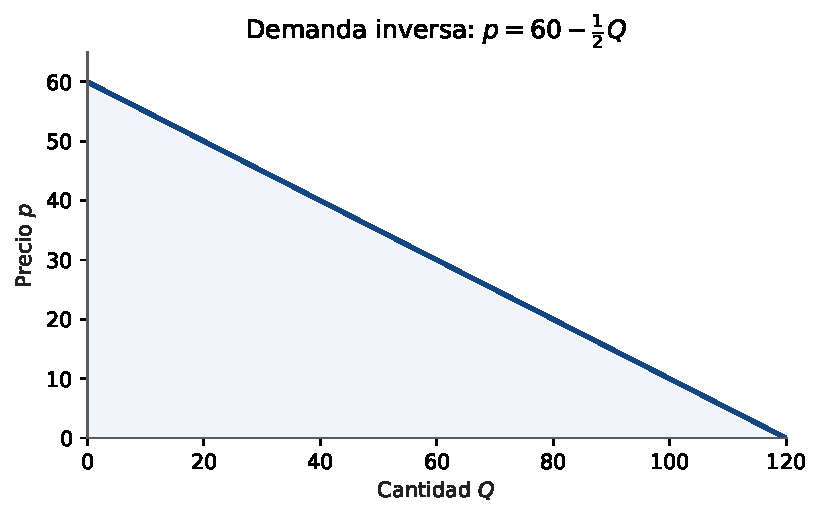
\includegraphics[width=0.72\linewidth]{figuras/demanda_inversa}
\caption{La demanda inversa expresa el precio máximo que el mercado paga por cada cantidad. El área bajo la curva representa la disposición total a pagar.}
\label{fig:demanda_inversa}
\end{figure}

\section{La función de oferta}

\begin{definicion}[Función de oferta]
La \emph{función de oferta} $Q_s = S(p)$ indica la cantidad que los productores están dispuestos a vender para cada precio $p$.
\end{definicion}

A diferencia de la demanda, la oferta suele ser \emph{creciente} en el precio: cuanto más alto el precio, más rentable producir y más unidades se ofrecen. Una forma lineal típica es
\begin{equation}
Q_s = c + d\,p, \qquad d>0.
\label{eq:oferta}
\end{equation}
El parámetro $c$ puede ser negativo: representa que por debajo de cierto precio mínimo no hay oferta (a nadie le conviene producir a pérdida).

\section{Costos: la estructura productiva}

Del lado de la empresa, la magnitud central es el \textbf{costo} de producir una cantidad $q$. Distinguimos:

\begin{itemize}
  \item \textbf{Costo fijo} ($CF$): no depende de la cantidad producida (alquiler, seguros, una máquina). Existe aunque $q=0$.
  \item \textbf{Costo variable} ($CV(q)$): crece con la producción (materia prima, energía, horas de trabajo).
  \item \textbf{Costo total}: $\;C(q) = CF + CV(q)$.
\end{itemize}

A partir del costo total se definen dos costos derivados de enorme importancia para la gestión:
\begin{align}
\text{Costo medio:}\quad & \cme(q) = \frac{C(q)}{q}, \label{eq:cme}\\[4pt]
\text{Costo marginal:}\quad & \cmg(q) = \frac{\dd C}{\dd q}. \label{eq:cmg}
\end{align}
El \textbf{costo medio} responde «¿cuánto me cuesta, en promedio, cada unidad?»; el \textbf{costo marginal} responde «¿cuánto me cuesta producir \emph{una unidad más}?». Volveremos sobre el costo marginal en el Capítulo~\ref{cap:marginal}, porque es una derivada y concentra buena parte de la lógica de las decisiones de producción \cite{nicholson}.

\section{Ingreso y beneficio}

\begin{definicion}[Ingreso total]
El \emph{ingreso total} es lo que la empresa factura: precio por cantidad,
\[
I(q) = p \cdot q.
\]
\end{definicion}

Si la empresa es precio-aceptante (vende a un precio $p$ fijo de mercado), el ingreso es una recta $I(q)=p\,q$. Pero si la empresa tiene poder de mercado y enfrenta la demanda inversa \eqref{eq:demanda_inversa}, el precio baja a medida que quiere vender más, y el ingreso se vuelve \emph{no lineal}:
\begin{equation}
I(q) = p(q)\cdot q = \left(\frac{a}{b} - \frac{1}{b}q\right) q .
\label{eq:ingreso}
\end{equation}

Finalmente, el objetivo habitual de la empresa:
\begin{equation}
\boxed{\;\Pi(q) = I(q) - C(q)\;}
\label{eq:beneficio}
\end{equation}
El \textbf{beneficio} (o utilidad económica) es la diferencia entre lo que entra y lo que sale. Maximizar $\Pi$ es el problema que resolveremos formalmente en el Capítulo~\ref{cap:optimizacion}; por ahora alcanza con tener clara la anatomía: ingreso menos costo.

\begin{ejemplo}[Armando las funciones de un kiosco]
Un kiosco enfrenta una demanda $Q_d = 120 - 2p$ (en unidades por día) y tiene un costo total $C(q) = 50 + 10q$ (en pesos). Entonces:
\begin{itemize}
  \item \emph{Demanda inversa:} despejando $p$, \; $p = 60 - \tfrac{1}{2}q$.
  \item \emph{Ingreso:} \; $I(q) = \left(60 - \tfrac12 q\right)q = 60q - \tfrac12 q^2$.
  \item \emph{Costo medio:} \; $\cme(q) = \dfrac{50+10q}{q} = \dfrac{50}{q} + 10$, que cae a medida que el costo fijo se reparte entre más unidades.
  \item \emph{Costo marginal:} \; $\cmg = 10$ (constante: cada unidad extra cuesta \$10).
  \item \emph{Beneficio:} \; $\Pi(q) = \big(60q - \tfrac12 q^2\big) - \big(50 + 10q\big) = -\tfrac12 q^2 + 50q - 50.$
\end{itemize}
Esta última es una parábola con las ramas hacia abajo: existe una cantidad que la maximiza, lo que anticipa el problema de optimización del Capítulo~\ref{cap:optimizacion}.
\end{ejemplo}

\begin{labbox}
En el laboratorio, estas funciones se representan con \texttt{sympy} (definiendo el símbolo \texttt{q} y escribiendo las expresiones tal cual aparecen acá) y se grafican con \texttt{matplotlib}. La traducción es directa: la ecuación \eqref{eq:beneficio} es, palabra por palabra, la línea \texttt{Pi = I - C} de la notebook. Graficar $\Pi(q)$ permite \emph{ver} dónde está el máximo antes de calcularlo, que es exactamente el puente entre la teoría de este capítulo y la práctica.
\end{labbox}

\section{Síntesis del capítulo}

Vimos que la actividad económica de una organización se describe con un puñado de funciones —demanda, oferta, costos, ingreso— y que de su combinación nace el beneficio. La demanda inversa, el costo marginal y el costo medio son los conceptos que más reaparecerán. En el próximo capítulo ponemos a interactuar demanda y oferta para encontrar el \emph{equilibrio de mercado}.

\chapter{Equilibrio de mercado y sistemas de ecuaciones}
\label{cap:equilibrio}

\section{El mercado como encuentro de dos fuerzas}

Un mercado pone en contacto a quienes quieren comprar (demanda) con quienes quieren vender (oferta). Cada lado reacciona al precio en sentido contrario: los compradores quieren precios bajos, los vendedores precios altos. La pregunta económica clásica es: \emph{¿existe un precio que concilie ambos deseos?} La respuesta es el \textbf{equilibrio de mercado}, una de las ideas más potentes de toda la economía y, según \cite{mankiw}, el verdadero «caballo de batalla» del análisis.

\begin{definicion}[Equilibrio de mercado]
El mercado está en \emph{equilibrio} en el par $(p^{*},q^{*})$ donde la cantidad demandada iguala a la ofrecida:
\[
Q_d(p^{*}) = Q_s(p^{*}) = q^{*}.
\]
A $p^{*}$ se lo llama \emph{precio de equilibrio} y a $q^{*}$ \emph{cantidad de equilibrio}.
\end{definicion}

La intuición del ajuste es la siguiente. Si el precio estuviera por encima de $p^{*}$, habría \emph{exceso de oferta} (sobra mercadería) y los vendedores bajarían precios. Si estuviera por debajo, habría \emph{exceso de demanda} (faltan productos, hay cola) y el precio subiría. Solo en $p^{*}$ no hay presión a moverse: por eso es un equilibrio.

\section{Resolver el equilibrio: un sistema de dos ecuaciones}

Encontrar el equilibrio es \textbf{resolver un sistema de ecuaciones}. Con la demanda \eqref{eq:demanda} y la oferta \eqref{eq:oferta}:
\begin{equation}
\begin{cases}
Q_d = a - b\,p \\[2pt]
Q_s = c + d\,p
\end{cases}
\qquad\Longrightarrow\qquad a - b\,p = c + d\,p .
\end{equation}
Igualando demanda y oferta y despejando, el precio de equilibrio es
\begin{equation}
p^{*} = \frac{a-c}{b+d}, \qquad\text{y luego}\qquad q^{*} = a - b\,p^{*}.
\label{eq:p_equilibrio}
\end{equation}

Esta es la versión más simple de un \textbf{sistema lineal}. Cuando los modelos crecen —varios mercados interconectados, varios bienes, restricciones— el sistema tiene más ecuaciones y más incógnitas, y conviene escribirlo en forma \emph{matricial} $A\mathbf{x}=\mathbf{b}$ y resolverlo con álgebra lineal, como veremos con Leontief en el Capítulo~\ref{cap:leontief}. La lógica, sin embargo, es siempre la misma: tantas ecuaciones independientes como incógnitas.

\begin{ejemplo}[Equilibrio en el mercado de un bien]
Sea $Q_d = 120 - 2p$ y $Q_s = -30 + 3p$. Igualando:
\[
120 - 2p = -30 + 3p \;\Longrightarrow\; 150 = 5p \;\Longrightarrow\; p^{*} = 30.
\]
La cantidad de equilibrio es $q^{*} = 120 - 2(30) = 60$. A un precio de \$30 se compran y venden exactamente 60 unidades, y el mercado se «vacía» sin sobrantes ni faltantes.
\end{ejemplo}

\begin{figure}[htbp]
\centering
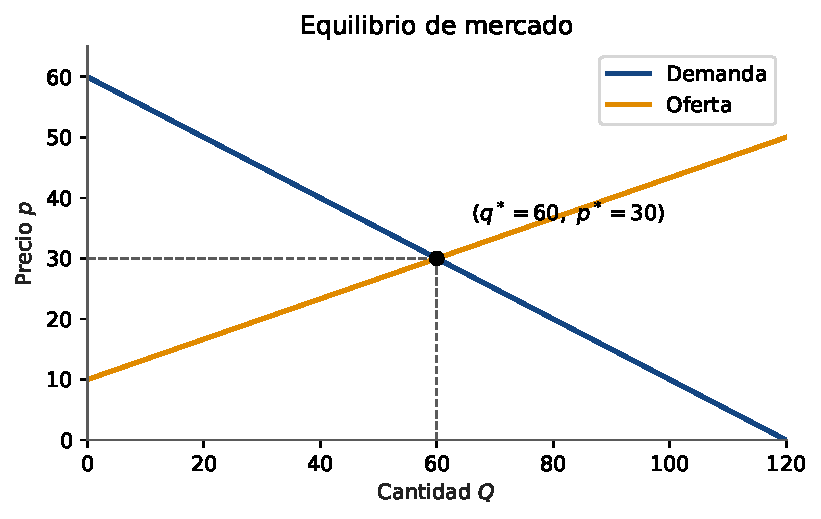
\includegraphics[width=0.72\linewidth]{figuras/equilibrio}
\caption{El equilibrio es la intersección de oferta y demanda. Por encima de $p^{*}$ sobra producto y el precio baja; por debajo, falta y el precio sube.}
\label{fig:equilibrio}
\end{figure}

\section{Estática comparativa: ¿qué pasa si algo cambia?}

El verdadero valor del equilibrio para la gestión no es el número en sí, sino poder responder \textbf{«¿qué pasaría si\ldots?»}. A este ejercicio se lo llama \emph{estática comparativa}: comparamos el equilibrio antes y después de un cambio en algún parámetro \cite{chiang}.

Por ejemplo, un impuesto específico de $t$ pesos por unidad cobrado al productor desplaza la oferta: ahora los vendedores necesitan $t$ pesos más por cada unidad, de modo que la oferta pasa a $Q_s = c + d(p - t)$. Recalculando \eqref{eq:p_equilibrio} se obtiene cómo cambian $p^{*}$ y $q^{*}$, y por lo tanto quién «paga» realmente el impuesto (la \emph{incidencia}). Este tipo de análisis —cambiar un parámetro y recomputar el equilibrio— es exactamente lo que las herramientas computacionales hacen sin esfuerzo, permitiendo explorar decenas de escenarios en segundos.

\begin{ideabox}
\textbf{Por qué importa.} El equilibrio convierte una pregunta de gestión vaga («¿conviene este precio?») en un cálculo reproducible. Y la estática comparativa convierte el modelo en una \emph{herramienta de simulación}: cambio un supuesto y veo el efecto. Esa es, en una frase, la promesa de los métodos cuantitativos aplicados.
\end{ideabox}

\begin{labbox}
En la notebook, resolver $Q_d = Q_s$ es una línea: \texttt{sympy.solve(Qd - Qs, p)}. La computadora despeja $p^{*}$ simbólicamente —sin que tengamos que hacer el álgebra a mano— y luego evalúa $q^{*}$. Para la estática comparativa basta cambiar un parámetro y volver a llamar a \texttt{solve}: el sistema de ecuaciones de \eqref{eq:p_equilibrio} se vuelve un experimento interactivo.
\end{labbox}

\section{Síntesis del capítulo}

El equilibrio de mercado surge de igualar oferta y demanda, lo que en términos matemáticos es resolver un sistema de ecuaciones. La estática comparativa nos permite estudiar el efecto de impuestos, subsidios o cambios de costos. En el próximo capítulo generalizamos la idea de «resolver sistemas» al caso de una economía con muchos sectores interdependientes: el modelo de Leontief.

\chapter{El modelo insumo-producto de Leontief}
\label{cap:leontief}

\section{Una economía es una red de sectores}

Hasta acá miramos un mercado por vez. Pero una economía real es una \textbf{red de sectores interdependientes}: para producir pan se necesita harina, para producir harina se necesita trigo y energía, y la energía a su vez consume insumos de otros sectores. Lo que es \emph{producto} de un sector es \emph{insumo} de otro. ¿Cómo planificar cuánto debe producir cada sector para abastecer tanto a los demás sectores como a la demanda final de los consumidores?

Wassily \textsc{Leontief} respondió esta pregunta con el \textbf{modelo insumo-producto}, un aporte que le valió el Premio Nobel de Economía en 1973 \cite{leontief}. Es, además, un bellísimo ejemplo de cómo el álgebra lineal —matrices y sistemas de ecuaciones— resuelve un problema económico que de otro modo sería inabordable.

\section{La matriz de coeficientes técnicos}

Supongamos $n$ sectores. La pieza central es la \textbf{matriz de coeficientes técnicos} $A$, cuyo elemento $a_{ij}$ indica \emph{cuántas unidades del sector $i$ se necesitan para producir una unidad del sector $j$}:
\begin{equation}
a_{ij} = \frac{\text{insumo del sector } i \text{ usado por } j}{\text{producción total del sector } j}.
\end{equation}
Cada columna $j$ de $A$ es, entonces, la «receta» del sector $j$: qué insumos y en qué proporción necesita.

Llamemos $\mathbf{x}$ al vector de producción total de cada sector y $\mathbf{d}$ al vector de \textbf{demanda final} (lo que consumen los hogares, el Estado y las exportaciones, por fuera de la cadena productiva). La identidad fundamental dice que \emph{toda la producción se reparte entre insumos intermedios y demanda final}:
\begin{equation}
\mathbf{x} = A\mathbf{x} + \mathbf{d}.
\label{eq:leontief_base}
\end{equation}
El término $A\mathbf{x}$ es lo que los sectores se consumen entre sí; $\mathbf{d}$ es lo que queda para la demanda final.

\section{La solución de Leontief}

La ecuación \eqref{eq:leontief_base} es un sistema lineal con $\mathbf{x}$ como incógnita. Reagrupando:
\begin{equation}
\mathbf{x} - A\mathbf{x} = \mathbf{d} \;\Longrightarrow\; (I - A)\mathbf{x} = \mathbf{d},
\end{equation}
donde $I$ es la matriz identidad. Si la matriz $(I-A)$ es invertible, la producción necesaria para satisfacer cualquier demanda final $\mathbf{d}$ es
\begin{equation}
\boxed{\;\mathbf{x} = (I - A)^{-1}\,\mathbf{d}\;}
\label{eq:leontief_sol}
\end{equation}
A la matriz $L = (I-A)^{-1}$ se la llama \textbf{matriz inversa de Leontief} o \textbf{matriz de requerimientos totales}. Su elemento $\ell_{ij}$ tiene una interpretación preciosa: cuánto debe producir el sector $i$, \emph{en forma directa e indirecta}, por cada unidad de demanda final del sector $j$. Captura los efectos en cadena que a simple vista no se ven.

\begin{ejemplo}[Una economía de dos sectores]
Sean dos sectores, Agro (1) e Industria (2), con matriz de coeficientes técnicos
\[
A = \begin{pmatrix} 0.2 & 0.3 \\ 0.4 & 0.1 \end{pmatrix},
\qquad
\mathbf{d} = \begin{pmatrix} 100 \\ 80 \end{pmatrix}.
\]
Entonces
\[
I - A = \begin{pmatrix} 0.8 & -0.3 \\ -0.4 & 0.9 \end{pmatrix}.
\]
El determinante es $\det(I-A) = (0.8)(0.9) - (-0.3)(-0.4) = 0.72 - 0.12 = 0.60$, y la inversa
\[
(I-A)^{-1} = \frac{1}{0.60}\begin{pmatrix} 0.9 & 0.3 \\ 0.4 & 0.8 \end{pmatrix}
= \begin{pmatrix} 1.5 & 0.5 \\ 0.667 & 1.333 \end{pmatrix}.
\]
La producción requerida es
\[
\mathbf{x} = (I-A)^{-1}\mathbf{d}
= \begin{pmatrix} 1.5(100)+0.5(80) \\ 0.667(100)+1.333(80) \end{pmatrix}
= \begin{pmatrix} 190 \\ 173.3 \end{pmatrix}.
\]
Es decir: para entregar 100 unidades de Agro y 80 de Industria a la demanda final, los sectores deben producir en total \(190\) y \(173.3\) unidades respectivamente. El excedente sobre la demanda final (90 y 93.3) es lo que se consume \emph{dentro} de la cadena productiva.
\end{ejemplo}

\begin{ideabox}
\textbf{Lectura de gestión.} El modelo de Leontief es la base de la planificación de la producción y del cálculo de \emph{multiplicadores} económicos: si la demanda de un sector crece, ¿cuánto debe crecer toda la economía para sostenerla? La matriz $(I-A)^{-1}$ contiene esa respuesta, efectos indirectos incluidos.
\end{ideabox}

\begin{labbox}
Acá el álgebra a mano se vuelve impracticable apenas hay más de dos o tres sectores: invertir una matriz $10\times 10$ es imposible con lápiz y papel pero instantáneo para una computadora. En el laboratorio se arma $A$ con \texttt{numpy}, se calcula \texttt{I - A} y la producción con \texttt{numpy.linalg.solve(I - A, d)} (numéricamente más estable que invertir y multiplicar). Es el ejemplo más claro de por qué necesitamos la máquina: la teoría cabe en una fórmula, pero el cálculo no cabe en una hoja.
\end{labbox}

\section{Una nota sobre el solapamiento con Álgebra}

Si ya cursaste Álgebra, parte de este capítulo te va a resultar familiar: la inversión de matrices y los sistemas lineales son contenido de esa materia. La diferencia —y el aporte de este curso— es la \textbf{interpretación económica}: acá una matriz no es un arreglo abstracto de números sino la radiografía de cómo una economía se produce a sí misma. Ese cambio de mirada, de la mecánica del cálculo al significado, es justamente lo que buscamos.

\section{Síntesis del capítulo}

El modelo de Leontief generaliza la idea de equilibrio a una economía con muchos sectores interdependientes, y la resuelve con la inversa $(I-A)^{-1}$. Con esto cerramos el bloque «estático» del curso. A partir del próximo capítulo incorporamos el \emph{cambio}: cómo medir variaciones con derivadas y por qué el pensamiento marginal está en el centro de toda decisión económica.

\chapter{Análisis marginal y derivadas}
\label{cap:marginal}

\section{Pensar «en el margen»}

Si hay una sola idea que distingue al razonamiento económico, es el \textbf{pensamiento marginal}: para decidir si hago \emph{un poco más} de algo, comparo el beneficio adicional con el costo adicional de esa unidad extra. No importa lo que ya gasté (eso es pasado, «costo hundido»); importa qué sumo y qué resto \emph{en el margen}. Mankiw lo enuncia como uno de sus diez principios de la economía: «las personas racionales piensan en términos marginales» \cite{mankiw}.

La herramienta matemática del pensamiento marginal es la \textbf{derivada}. Por eso este capítulo es, a la vez, un repaso de cálculo y una de las claves conceptuales del curso.

\section{La derivada como tasa de cambio}

\begin{definicion}[Derivada]
La \emph{derivada} de una función $f$ en un punto $x$ mide la tasa instantánea a la que $f$ cambia ante un cambio infinitesimal de $x$:
\[
f'(x) = \frac{\dd f}{\dd x} = \lim_{h\to 0}\frac{f(x+h)-f(x)}{h}.
\]
Geométricamente, es la \emph{pendiente} de la recta tangente a la curva en ese punto.
\end{definicion}

La lectura económica es directa: la derivada responde «si aumento $x$ en una unidad pequeña, ¿cuánto cambia $f$?». Recordemos algunas reglas que usaremos sin demostrar (están en cualquier manual de matemática para economistas, p. ej. \cite{sydsaeter}):
\[
\frac{\dd}{\dd q}(q^n) = n\,q^{\,n-1}, \qquad
\frac{\dd}{\dd q}(k) = 0, \qquad
\frac{\dd}{\dd q}\big(u(q)\pm v(q)\big) = u'(q)\pm v'(q).
\]

\section{Costo, ingreso y beneficio marginales}

Aplicando la derivada a las funciones del Capítulo~\ref{cap:funciones} obtenemos las magnitudes marginales:
\begin{align}
\text{Costo marginal:}\quad & \cmg(q) = C'(q) = \frac{\dd C}{\dd q}, \\[3pt]
\text{Ingreso marginal:}\quad & \img(q) = I'(q) = \frac{\dd I}{\dd q}, \\[3pt]
\text{Beneficio marginal:}\quad & \Pi'(q) = \img(q) - \cmg(q).
\end{align}
La última igualdad encierra la regla de oro de la producción: \emph{conviene producir una unidad más mientras el ingreso marginal supere al costo marginal} ($\img > \cmg$), porque esa unidad agrega más de lo que cuesta. El óptimo se alcanza cuando se igualan, $\img = \cmg$, idea que formalizamos en el Capítulo~\ref{cap:optimizacion}.

\begin{ejemplo}[Del costo total al costo marginal]
Sea $C(q) = 50 + 10q + 0.5q^2$. Derivando término a término:
\[
\cmg(q) = C'(q) = 10 + q.
\]
El costo de la primera unidad es aproximadamente $\cmg(1)=11$, y el de la unidad número 20 es $\cmg(20)=30$: el costo marginal crece, reflejando rendimientos decrecientes. Notá que el costo fijo (50) \emph{desaparece} al derivar: lo fijo no afecta la decisión marginal, coherente con la intuición de que los costos hundidos no deben pesar en el margen.
\end{ejemplo}

\section{La relación entre lo marginal y lo medio}

Una propiedad que confunde al principio pero es muy útil: \textbf{el marginal arrastra al medio}. Cuando el valor marginal está por debajo del promedio, el promedio cae; cuando está por encima, el promedio sube; y se cruzan en el mínimo (o máximo) del promedio. Es la misma lógica que las notas: si te sacás en un parcial menos que tu promedio, el promedio baja.

Formalmente, derivando el costo medio $\cme(q)=C(q)/q$ con la regla del cociente:
\begin{equation}
\frac{\dd \cme}{\dd q} = \frac{C'(q)\,q - C(q)}{q^2} = \frac{1}{q}\big(\cmg(q) - \cme(q)\big).
\end{equation}
El signo de esta derivada depende de si $\cmg \gtrless \cme$: el costo medio decrece mientras el marginal esté por debajo y crece cuando lo supera, alcanzando su mínimo justo donde $\cmg = \cme$. Esta es la razón teórica de la típica curva de costo medio en forma de U \cite{nicholson}.

\begin{figure}[htbp]
\centering
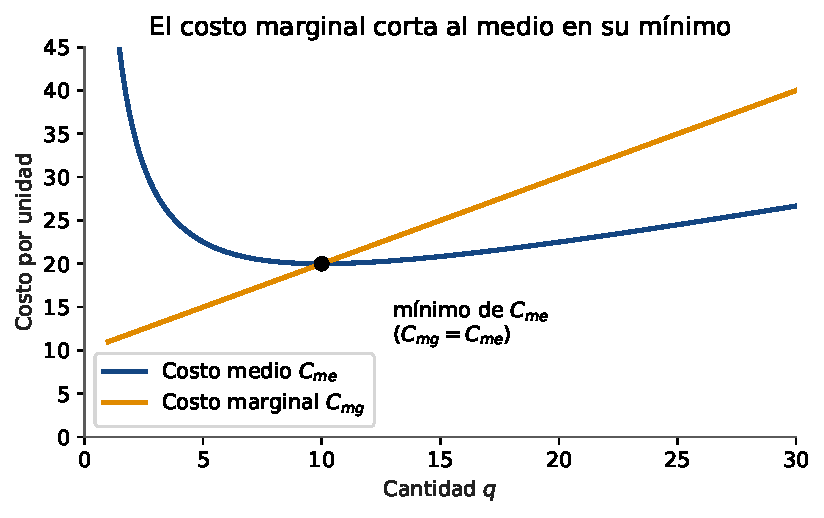
\includegraphics[width=0.72\linewidth]{figuras/costos_U}
\caption{El costo marginal corta al costo medio exactamente en el mínimo de este último: mientras $\cmg<\cme$ el promedio baja; cuando $\cmg>\cme$, sube.}
\label{fig:costos_U}
\end{figure}

\begin{ideabox}
\textbf{Por qué importa para la gestión.} El análisis marginal evita dos errores caros: producir de más (cuando cada unidad nueva cuesta más de lo que rinde) y obsesionarse con costos hundidos. La pregunta correcta nunca es «¿cuánto gasté?», sino «¿qué me suma y qué me cuesta la próxima unidad?».
\end{ideabox}

\begin{labbox}
En el laboratorio, derivar es una sola instrucción: \texttt{sympy.diff(C, q)} devuelve el costo marginal simbólicamente, sin reglas memorizadas. Esto permite obtener $\cmg$, $\img$ y $\Pi'$ a partir de las funciones del capítulo anterior y graficarlas para \emph{ver} dónde el beneficio marginal se hace cero. La computadora hace el cálculo; lo que aporta el economista es saber \emph{qué} derivar y \emph{cómo} interpretarlo.
\end{labbox}

\section{Síntesis del capítulo}

La derivada traduce el pensamiento marginal en cálculo: costo, ingreso y beneficio marginales son derivadas de sus respectivas funciones totales. La relación marginal–medio explica la forma de las curvas de costo. Con la derivada como herramienta de medición del cambio, en el próximo capítulo construimos un concepto que es pura «sensibilidad relativa»: la elasticidad.

\chapter{Elasticidades: medir la sensibilidad}
\label{cap:elasticidad}

\section{El problema de las unidades}

Sabemos que si sube el precio, baja la cantidad demandada (Capítulo~\ref{cap:funciones}). Pero, ¿cuánto? La derivada $\dd Q/\dd p$ da una respuesta, con un problema: \textbf{depende de las unidades}. Si mido la cantidad en kilos o en toneladas, o el precio en pesos o en dólares, el número cambia, aunque la realidad económica sea la misma. Para comparar sensibilidades entre productos y mercados necesitamos una medida \emph{sin unidades}. Esa medida es la \textbf{elasticidad}: el cociente de \emph{variaciones porcentuales} \cite{varian}.

\section{Elasticidad precio de la demanda}

\begin{definicion}[Elasticidad precio de la demanda]
Es la variación porcentual de la cantidad demandada ante una variación porcentual del precio:
\[
\varepsilon = \frac{\%\,\Delta Q}{\%\,\Delta p}
= \frac{\dd Q}{\dd p}\cdot\frac{p}{Q}.
\]
\end{definicion}

Como la demanda es decreciente, $\varepsilon$ es normalmente negativa; por comodidad se suele hablar de su valor absoluto $|\varepsilon|$. La clasificación clave para la gestión es:
\begin{itemize}
  \item $|\varepsilon| > 1$: demanda \textbf{elástica}. La cantidad reacciona \emph{más} que proporcionalmente al precio (bienes con sustitutos, lujos).
  \item $|\varepsilon| < 1$: demanda \textbf{inelástica}. La cantidad reacciona \emph{menos} que proporcionalmente (bienes de primera necesidad, sin sustitutos).
  \item $|\varepsilon| = 1$: elasticidad \textbf{unitaria}.
\end{itemize}

\subsection*{Elasticidad punto y elasticidad arco}

La fórmula anterior es la elasticidad \emph{puntual} (en un precio dado, usando la derivada). Cuando solo tenemos dos puntos observados —dos pares (precio, cantidad)— se usa la elasticidad \emph{arco}, que toma como base el promedio de ambos puntos para evitar que el resultado dependa de cuál tomamos como inicial:
\begin{equation}
\varepsilon_{\text{arco}} = \frac{\Delta Q/\big[(Q_1+Q_2)/2\big]}{\Delta p/\big[(p_1+p_2)/2\big]}.
\end{equation}

\section{Elasticidad e ingreso total: la regla que todo gerente debería saber}

¿Conviene subir el precio? La respuesta depende de la elasticidad, a través de su efecto sobre el \textbf{ingreso total} $I = p\cdot Q$. Hay dos fuerzas opuestas: subir $p$ aumenta el ingreso por unidad, pero reduce las unidades $Q$. Quién gana define la elasticidad:

\begin{center}
\begin{tabular}{lll}
\toprule
\textbf{Si la demanda es\ldots} & \textbf{y subo el precio\ldots} & \textbf{el ingreso total\ldots} \\
\midrule
Elástica ($|\varepsilon|>1$)    & $p\uparrow$ & \emph{baja} (manda la caída de $Q$) \\
Inelástica ($|\varepsilon|<1$)  & $p\uparrow$ & \emph{sube} (manda la suba de $p$) \\
Unitaria ($|\varepsilon|=1$)    & $p\uparrow$ & no cambia (ingreso máximo) \\
\bottomrule
\end{tabular}
\end{center}

Formalmente, el ingreso marginal se relaciona con la elasticidad mediante
\begin{equation}
\img = p\left(1 + \frac{1}{\varepsilon}\right),
\label{eq:img_elasticidad}
\end{equation}
de donde el ingreso total es máximo cuando $\img=0$, es decir cuando $\varepsilon=-1$ (elasticidad unitaria). Este resultado conecta directamente con la optimización del Capítulo~\ref{cap:optimizacion}: una empresa con poder de mercado nunca opera en el tramo inelástico de su demanda, porque ahí todavía podría subir el precio y ganar más \cite{pindyck}.

\begin{ejemplo}[¿Subo el precio del café?]
Una cafetería vende $Q = 200 - 10p$ tazas por día. En $p=8$: $Q=120$. La elasticidad puntual es
\[
\varepsilon = \frac{\dd Q}{\dd p}\cdot\frac{p}{Q} = (-10)\cdot\frac{8}{120} = -0.667.
\]
Como $|\varepsilon| = 0.667 < 1$, la demanda es \emph{inelástica} a ese precio: subir el precio aumentaría el ingreso. El ingreso se maximiza donde $\varepsilon=-1$; resolviendo $(-10)\,p/(200-10p) = -1$ se obtiene $p=10$, con $Q=100$ e ingreso $I=1000$, mayor que los \$960 que se facturan a $p=8$.
\end{ejemplo}

\begin{figure}[htbp]
\centering
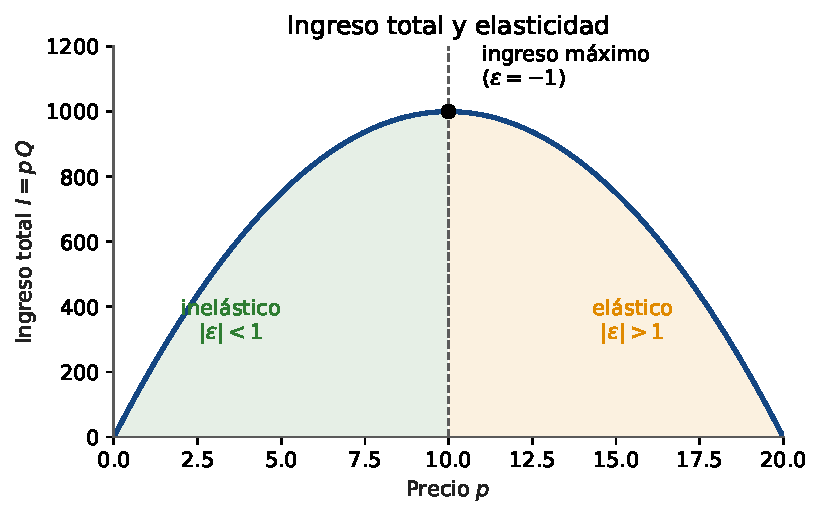
\includegraphics[width=0.72\linewidth]{figuras/elasticidad_ingreso}
\caption{El ingreso total alcanza su máximo cuando la elasticidad es unitaria ($\varepsilon=-1$). En el tramo inelástico conviene subir el precio; en el elástico, bajarlo.}
\label{fig:elasticidad_ingreso}
\end{figure}

\section{Otras elasticidades}

El concepto se extiende a cualquier par de variables:
\begin{itemize}
  \item \textbf{Elasticidad ingreso de la demanda} $\varepsilon_R = \dfrac{\%\,\Delta Q}{\%\,\Delta R}$ (respecto al ingreso $R$ del consumidor): positiva para bienes \emph{normales}, negativa para bienes \emph{inferiores}.
  \item \textbf{Elasticidad cruzada} $\varepsilon_{xy} = \dfrac{\%\,\Delta Q_x}{\%\,\Delta p_y}$: positiva si los bienes son \emph{sustitutos} (sube el precio del té, subo el consumo de café), negativa si son \emph{complementarios} (sube el precio de la nafta, baja el uso del auto).
\end{itemize}

\begin{ideabox}
\textbf{Por qué importa.} La elasticidad es probablemente el concepto micro más usado en la gestión real: define estrategias de precios, el efecto de un impuesto, la conveniencia de una promoción. Y como es adimensional, permite comparar la sensibilidad de productos tan distintos como la sal y los pasajes de avión.
\end{ideabox}

\begin{labbox}
En la práctica, la elasticidad puntual combina una derivada (\texttt{sympy.diff}) con una evaluación en un punto; la elasticidad arco se calcula directo a partir de dos filas de un \texttt{DataFrame} de \texttt{pandas} con datos reales de precios y cantidades. El curso suele pedir estimarla sobre datos observados: ahí la teoría de este capítulo se encuentra con los datos del laboratorio.
\end{labbox}

\section{Síntesis del capítulo}

La elasticidad mide sensibilidad en términos porcentuales, lo que la hace comparable entre mercados. Su relación con el ingreso total es una herramienta directa de decisión de precios. En el próximo capítulo pasamos de la derivada (medir el cambio) a su operación inversa, la integral (acumular el cambio), para medir el bienestar.

\chapter{Integrales y excedentes económicos}
\label{cap:integrales}

\section{La operación inversa de la derivada}

Si la derivada \emph{desarma} un total en su ritmo de cambio (del costo total al costo marginal), la \textbf{integral} hace lo contrario: \emph{rearma} el total a partir del ritmo de cambio. Conocido el costo marginal, integrando recuperamos el costo total; conocido el ingreso marginal, recuperamos el ingreso. Esta dualidad —el Teorema Fundamental del Cálculo— es la que nos permitirá medir áreas con significado económico \cite{chiang}.

\begin{definicion}[Integral definida]
La \emph{integral definida} de una función $f$ entre $a$ y $b$ es el área (con signo) bajo la curva $f$ en ese intervalo:
\[
\int_a^b f(x)\dd x .
\]
Si $F$ es una primitiva de $f$ (es decir, $F'=f$), entonces $\displaystyle\int_a^b f(x)\dd x = F(b)-F(a)$.
\end{definicion}

\section{Recuperar totales a partir de marginales}

Como el costo marginal es la derivada del costo total, integrarlo lo reconstruye:
\begin{equation}
C(q) = \int_0^q \cmg(u)\dd u + CF.
\label{eq:costo_desde_cmg}
\end{equation}
Acá aparece un detalle conceptual importante y fuente de errores frecuentes: \textbf{la integral recupera la parte variable, pero no el costo fijo}. La integración deja indeterminada una constante, y esa constante es justamente el costo fijo $CF$, que hay que sumar aparte porque no proviene de producir unidades. Para el ingreso, en cambio, la condición natural $I(0)=0$ (no vender no genera ingreso) fija la constante en cero.

\begin{ejemplo}[Del costo marginal al costo total]
Si $\cmg(q) = 10 + q$ y el costo fijo es $CF=50$, entonces
\[
C(q) = \int_0^q (10+u)\dd u + 50 = \Big[10u + \tfrac{u^2}{2}\Big]_0^q + 50 = 10q + \tfrac{q^2}{2} + 50,
\]
que es exactamente la función de costo total del Ejemplo del Capítulo~\ref{cap:marginal}. La derivada y la integral son, en efecto, caminos de ida y vuelta.
\end{ejemplo}

\section{El excedente del consumidor}

Acá la integral despliega todo su valor económico. Recordemos la demanda inversa $p(Q)$: indica el \emph{máximo} precio que alguien está dispuesto a pagar por cada unidad. Las primeras unidades se valoran mucho (precio de reserva alto); las últimas, menos. Pero en el mercado \emph{todas} se pagan al mismo precio de equilibrio $p^{*}$. La diferencia entre lo que la gente \emph{estaba dispuesta a pagar} y lo que \emph{efectivamente pagó} es una ganancia neta de bienestar para los consumidores.

\begin{definicion}[Excedente del consumidor]
Es el área entre la curva de demanda inversa y el precio de equilibrio, entre $0$ y la cantidad de equilibrio:
\[
EC = \int_0^{q^{*}} \big(p_d(Q) - p^{*}\big)\dd Q .
\]
\end{definicion}

\section{El excedente del productor}

Simétricamente, la oferta inversa $p_s(Q)$ indica el \emph{mínimo} precio al que los productores aceptan vender cada unidad (su costo marginal). Si el precio de mercado supera ese mínimo, el productor gana la diferencia.

\begin{definicion}[Excedente del productor]
Es el área entre el precio de equilibrio y la curva de oferta inversa:
\[
EP = \int_0^{q^{*}} \big(p^{*} - p_s(Q)\big)\dd Q .
\]
\end{definicion}

La suma $EC + EP$ es el \textbf{excedente total} o bienestar que el mercado genera. Aquí conviene una advertencia que el curso remarca: integrar directamente la diferencia entre demanda y oferta, $\int_0^{q^{*}}(p_d - p_s)\dd Q$, da el excedente \emph{total}, no el del consumidor; para separar $EC$ y $EP$ hay que usar el precio de equilibrio $p^{*}$ como frontera entre ambas áreas.

\begin{ejemplo}[Excedentes en un mercado lineal]
Con demanda inversa $p_d = 60 - \tfrac12 Q$ y equilibrio en $q^{*}=60$, $p^{*}=30$:
\[
EC = \int_0^{60}\Big(60 - \tfrac12 Q - 30\Big)\dd Q
= \int_0^{60}\Big(30 - \tfrac12 Q\Big)\dd Q
= \Big[30Q - \tfrac{Q^2}{4}\Big]_0^{60} = 1800 - 900 = 900.
\]
El excedente del consumidor es de \$900 por día: es el «valor regalado» que reciben los compradores por pagar \$30 unidades que muchos hubieran pagado más caras. Geométricamente, es el triángulo entre la demanda y la línea de precio.
\end{ejemplo}

\begin{figure}[htbp]
\centering
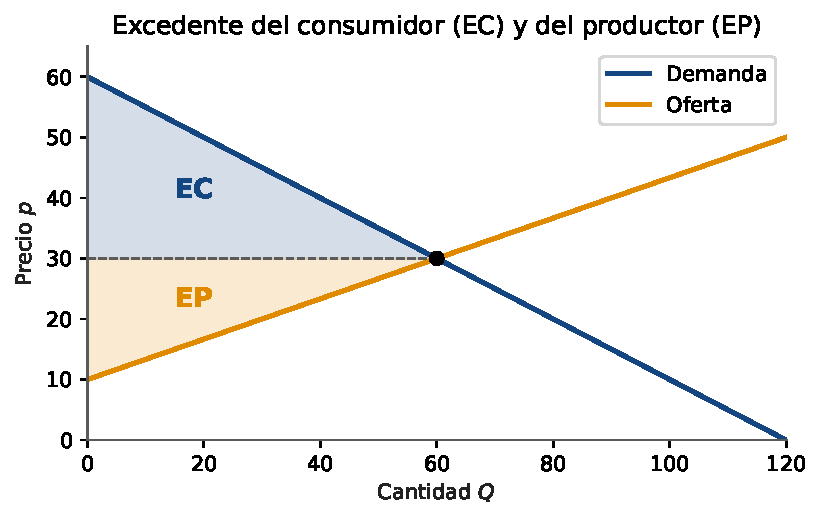
\includegraphics[width=0.72\linewidth]{figuras/excedentes}
\caption{El excedente del consumidor (EC) es el área entre la demanda y el precio; el del productor (EP), entre el precio y la oferta. Su suma es el bienestar total del mercado.}
\label{fig:excedentes}
\end{figure}

\begin{ideabox}
\textbf{Por qué importa.} Los excedentes son la forma en que la economía \emph{mide el bienestar}. Permiten evaluar políticas (un impuesto, un control de precios, una fusión) en términos de cuánto ganan o pierden consumidores y productores. Es el puente entre la microeconomía positiva («qué pasa») y la normativa («qué conviene»).
\end{ideabox}

\begin{labbox}
En el laboratorio, integrar es \texttt{sympy.integrate(f, (Q, a, b))}. El excedente del consumidor sale de integrar la demanda inversa menos el precio de equilibrio; el del productor, el precio menos la oferta inversa. Recordá la trampa: \texttt{sympy.integrate} no agrega la constante, así que para reconstruir el costo total hay que sumar el costo fijo a mano, tal como en la ecuación~\eqref{eq:costo_desde_cmg}.
\end{labbox}

\section{Síntesis del capítulo}

La integral acumula: reconstruye totales a partir de marginales y, sobre todo, mide los excedentes que cuantifican el bienestar de consumidores y productores. Con derivadas (medir el cambio) e integrales (acumularlo) ya tenemos todo el cálculo necesario para abordar el problema central de la empresa: optimizar.

\chapter{Optimización económica}
\label{cap:optimizacion}

\section{Decidir es optimizar}

Toda la teoría de la empresa converge en una pregunta: \emph{¿cuánto producir para ganar lo más posible?} Optimizar es buscar el valor de una variable de decisión —la cantidad, el precio, la combinación de productos— que hace máxima (o mínima) una función objetivo. Con el cálculo del Capítulo~\ref{cap:marginal} ya tenemos la llave: en un máximo «liso», la pendiente de la función objetivo es cero \cite{chiang}.

\section{Optimización libre: el máximo beneficio}

Queremos maximizar el beneficio $\Pi(q) = I(q) - C(q)$. El procedimiento tiene dos pasos.

\paragraph{Condición de primer orden (CPO).} En el óptimo, la derivada se anula:
\begin{equation}
\Pi'(q^{*}) = 0 \;\Longleftrightarrow\; I'(q^{*}) = C'(q^{*}) \;\Longleftrightarrow\; \boxed{\img = \cmg}.
\label{eq:cpo}
\end{equation}
Reencontramos, ahora con todo rigor, la regla anticipada en capítulos anteriores: \textbf{se produce hasta que el ingreso marginal iguala al costo marginal}. La intuición es imbatible: mientras $\img > \cmg$, cada unidad extra agrega beneficio; cuando $\img < \cmg$, resta. El punto de quiebre es el óptimo.

\paragraph{Condición de segundo orden (CSO).} La CPO también la cumpliría un \emph{mínimo}. Para asegurar que es un máximo, la función debe ser cóncava ahí: la segunda derivada negativa,
\begin{equation}
\Pi''(q^{*}) < 0.
\label{eq:cso}
\end{equation}

\begin{ejemplo}[El beneficio máximo del kiosco]
Retomemos $\Pi(q) = -\tfrac12 q^2 + 50q - 50$ del Capítulo~\ref{cap:funciones}. La CPO:
\[
\Pi'(q) = -q + 50 = 0 \;\Longrightarrow\; q^{*} = 50.
\]
La CSO: $\Pi''(q) = -1 < 0$, así que es efectivamente un máximo. El beneficio óptimo es
\[
\Pi(50) = -\tfrac12(2500) + 50(50) - 50 = -1250 + 2500 - 50 = 1200.
\]
Producir 50 unidades diarias maximiza el beneficio en \$1200. Ni una más (empezaría a perder en el margen), ni una menos (dejaría ganancia sobre la mesa).
\end{ejemplo}

\begin{figure}[htbp]
\centering
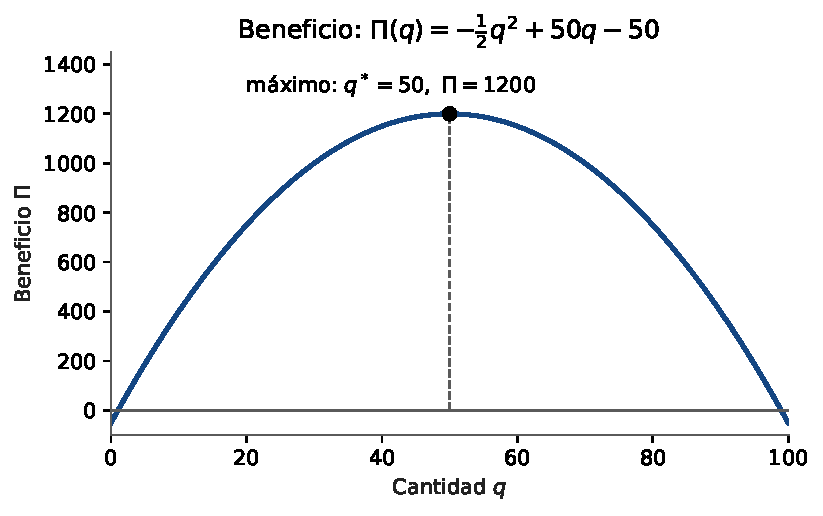
\includegraphics[width=0.72\linewidth]{figuras/beneficio}
\caption{La función de beneficio es una parábola cóncava: su vértice (donde la pendiente es cero, $\Pi'=0$) marca la cantidad que maximiza la ganancia.}
\label{fig:beneficio}
\end{figure}

\section{Optimización con restricciones: cuando los recursos son escasos}

En la gestión real rara vez se decide una sola cantidad sin límites. Lo habitual es elegir \emph{cuánto producir de varios productos} con \textbf{recursos limitados}: horas de máquina, presupuesto, materia prima. Esto es un problema de \emph{optimización con restricciones}, y cuando tanto el objetivo como las restricciones son lineales, se llama \textbf{programación lineal}.

Su forma general: elegir cantidades $x_1,\dots,x_n$ que
\begin{equation}
\max\ \ Z = \sum_{j} c_j x_j
\qquad\text{sujeto a}\qquad
\sum_{j} a_{ij}\,x_j \le b_i,\quad x_j \ge 0,
\end{equation}
donde $c_j$ es el margen de cada producto, $a_{ij}$ cuánto recurso $i$ consume el producto $j$, y $b_i$ la disponibilidad del recurso $i$. La solución óptima siempre se encuentra en un \emph{vértice} de la región factible —el polígono de combinaciones que respetan todas las restricciones—, resultado central de la teoría de la programación lineal.

\begin{ejemplo}[Mezcla de producción]
Una fábrica produce sillas ($x_1$, margen \$40) y mesas ($x_2$, margen \$60). Cada silla usa 2~h de carpintería y cada mesa 4~h; hay 100~h disponibles. Además se dispone de 80~h de pintura, con 1~h por silla y 1~h por mesa. El problema es
\[
\max\ \ 40x_1 + 60x_2 \quad\text{s.a.}\quad 2x_1+4x_2\le 100,\ \ x_1+x_2\le 80,\ \ x_1,x_2\ge 0.
\]
La solución óptima asigna las horas escasas al producto que más margen aporta por hora de recurso. Resolverlo a mano con dos productos es viable; con decenas de productos y restricciones se vuelve imposible, y por eso recurrimos a la computadora.
\end{ejemplo}

\begin{labbox}
Dos herramientas, según el problema. Para la \emph{optimización libre} (máximo beneficio), el laboratorio usa \texttt{sympy}: derivar el beneficio y resolver $\Pi'(q)=0$ con \texttt{sympy.solve(sympy.diff(I-C, q), q)}, verificando el signo de la segunda derivada. Para la \emph{optimización con restricciones}, se usa \texttt{PuLP}: se declaran las variables, la función objetivo y las restricciones casi con las mismas palabras de la formulación matemática, y el \emph{solver} encuentra el vértice óptimo. La fórmula~\eqref{eq:cpo} y el método de \texttt{PuLP} son las dos caras —cálculo y álgebra lineal— de la misma idea de optimizar.
\end{labbox}

\begin{ideabox}
\textbf{Por qué importa.} La optimización es el punto donde la economía deja de describir y empieza a \emph{recomendar}: dado un objetivo y unas restricciones, dice cuál es la mejor decisión posible. Es el corazón cuantitativo de la gestión.
\end{ideabox}

\section{Síntesis del capítulo}

Maximizar el beneficio lleva a la regla $\img=\cmg$ (CPO), validada por la concavidad (CSO). Cuando hay recursos escasos y varios productos, la programación lineal generaliza el problema. En el próximo capítulo aplicamos la optimización a un escenario estratégico: dos empresas que compiten y deben anticipar la decisión de la rival.

\chapter{Competencia imperfecta: el duopolio de Cournot}
\label{cap:duopolio}

\section{Entre el monopolio y la competencia}

Hasta acá la empresa decidía sola. Pero muchos mercados reales están dominados por \emph{pocas} empresas grandes (un \textbf{oligopolio}): telefonía, combustibles, supermercados. Ahí aparece algo nuevo y fascinante: el beneficio de cada empresa depende también de lo que haga la otra. Decidir se vuelve \textbf{estratégico} —hay que anticipar al rival—, y la herramienta para pensarlo es la \emph{teoría de juegos} \cite{gibbons}.

El modelo más clásico es el \textbf{duopolio de Cournot} (Augustin Cournot, 1838): dos empresas producen un bien homogéneo y compiten eligiendo \emph{cantidades} de forma simultánea. El precio de mercado surge de la cantidad total ofrecida.

\section{El problema de cada empresa}

Sean dos empresas con cantidades $q_1$ y $q_2$. La cantidad total es $Q = q_1 + q_2$ y el precio lo fija la demanda inversa del mercado, por ejemplo lineal:
\begin{equation}
p(Q) = a - b\,(q_1 + q_2).
\end{equation}
Si cada empresa tiene costo marginal constante $c$, el beneficio de la empresa 1 es
\begin{equation}
\Pi_1(q_1,q_2) = \big[a - b(q_1+q_2)\big]q_1 - c\,q_1 .
\end{equation}
Lo decisivo: $\Pi_1$ depende de $q_2$, que la empresa 1 \emph{no controla}. Lo que sí puede hacer es elegir su mejor $q_1$ \emph{para cada} valor posible de $q_2$.

\section{La función de mejor respuesta}

La empresa 1 maximiza su beneficio tomando $q_2$ como dado. Aplicando la CPO del Capítulo~\ref{cap:optimizacion} (derivar respecto de $q_1$ e igualar a cero):
\begin{equation}
\frac{\partial \Pi_1}{\partial q_1} = a - 2b\,q_1 - b\,q_2 - c = 0
\;\Longrightarrow\;
q_1 = \frac{a - c - b\,q_2}{2b}.
\label{eq:mejor_respuesta}
\end{equation}
Esta es la \textbf{función de mejor respuesta} (o reacción) de la empresa 1: su producción óptima \emph{en función} de lo que produzca la 2. Cuanto más produce la rival, menos le conviene producir a ella (las cantidades son «sustitutos estratégicos»). Por simetría, la empresa 2 tiene su propia mejor respuesta.

\section{El equilibrio de Nash-Cournot}

¿Dónde termina esta mutua anticipación? En el punto en que \textbf{ninguna empresa quiere cambiar su decisión dada la de la otra}: ambas están sobre su mejor respuesta a la vez. Eso es un \textbf{equilibrio de Nash} \cite{gibbons}. Por simetría $q_1^{*}=q_2^{*}=q^{*}$, y reemplazando en \eqref{eq:mejor_respuesta}:
\begin{equation}
q^{*} = \frac{a-c}{3b}, \qquad Q^{*} = 2q^{*} = \frac{2(a-c)}{3b}.
\end{equation}

\begin{ejemplo}[Un duopolio concreto]
Sea $p = 100 - (q_1+q_2)$ (es decir $a=100$, $b=1$) y costo marginal $c=10$. La mejor respuesta de la empresa 1 es $q_1 = (90 - q_2)/2$. En el equilibrio simétrico:
\[
q^{*} = \frac{100-10}{3} = 30, \qquad Q^{*} = 60, \qquad p^{*} = 100 - 60 = 40.
\]
El beneficio de cada empresa es $\Pi = (40-10)\cdot 30 = 900$.
\end{ejemplo}

\begin{figure}[htbp]
\centering
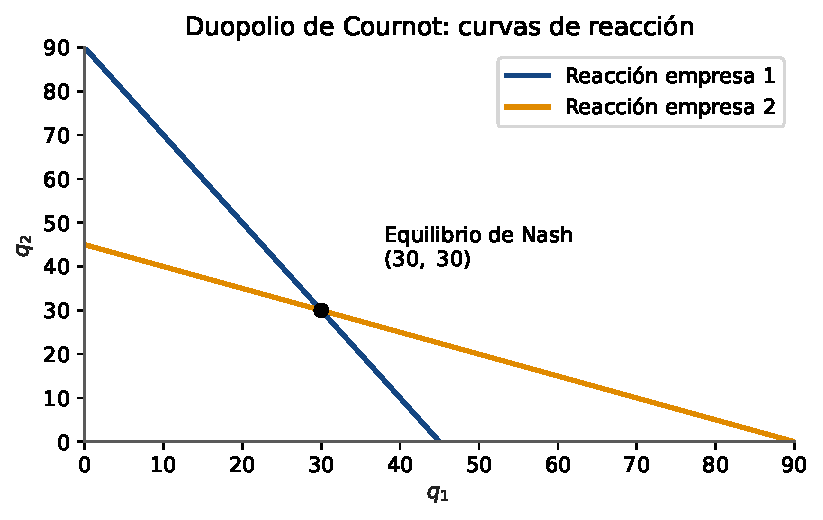
\includegraphics[width=0.72\linewidth]{figuras/cournot}
\caption{Las curvas de reacción de ambas empresas. Donde se cruzan, cada una está dando su mejor respuesta a la otra: ese punto es el equilibrio de Nash-Cournot.}
\label{fig:cournot}
\end{figure}

\section{Comparación: ¿cuánto importa la estructura del mercado?}

La gracia del modelo es comparar el duopolio con los dos extremos, usando los mismos números ($a=100$, $b=1$, $c=10$):

\begin{center}
\begin{tabular}{lccc}
\toprule
\textbf{Estructura} & \textbf{Cantidad total $Q$} & \textbf{Precio $p$} & \textbf{Beneficio total} \\
\midrule
Monopolio        & 45 & 55 & 2025 \\
Duopolio Cournot & 60 & 40 & 1800 \\
Competencia perfecta & 90 & 10 & 0 \\
\bottomrule
\end{tabular}
\end{center}

El patrón es nítido: a medida que aumenta la competencia (de 1 a 2 a muchas empresas), \textbf{la cantidad total sube, el precio baja y se acerca al costo marginal, y el beneficio extraordinario se disipa}. El consumidor gana con la competencia; las empresas la resisten. El duopolio queda, como era de esperar, a mitad de camino \cite{pindyck}. Con $n$ empresas idénticas, puede mostrarse que $Q = \tfrac{n}{n+1}\cdot\tfrac{a-c}{b}$, que tiende al resultado competitivo cuando $n\to\infty$.

\begin{ideabox}
\textbf{Por qué importa.} La teoría de juegos explica fenómenos que el modelo de empresa aislada no puede: guerras de precios, colusión, barreras de entrada, decisiones de capacidad. Es la base del análisis de la competencia y de la política antimonopolio (la «defensa de la competencia»).
\end{ideabox}

\begin{labbox}
En el laboratorio, el equilibrio de Cournot se resuelve planteando las dos funciones de mejor respuesta como un \emph{sistema de ecuaciones} y usando \texttt{sympy.solve} sobre $q_1$ y $q_2$ a la vez —es, otra vez, resolver un sistema, como en el Capítulo~\ref{cap:equilibrio}—. También puede graficarse el cruce de las dos curvas de reacción: el punto donde se cortan es el equilibrio de Nash. La teoría estratégica se vuelve, así, dos rectas que se intersecan en la pantalla.
\end{labbox}

\section{Síntesis del capítulo}

Cuando pocas empresas interactúan, decidir es anticipar. La función de mejor respuesta y el equilibrio de Nash resuelven el duopolio de Cournot, que se ubica entre el monopolio y la competencia perfecta. En el capítulo final pasamos del corto plazo de la producción al largo plazo de las decisiones de inversión.

\chapter{Evaluación de proyectos de inversión}
\label{cap:inversiones}

\section{Plata hoy no es plata mañana}

Invertir es resignar dinero hoy a cambio de flujos futuros inciertos: comprar una máquina, abrir una sucursal, lanzar un producto. La pregunta de gestión es \emph{¿conviene?}, y para responderla hace falta un principio que parece obvio pero lo cambia todo: \textbf{un peso hoy vale más que un peso dentro de un año}. Por tres razones —puedo invertirlo y ganar interés, la inflación le quita poder de compra, y el futuro es incierto— el dinero tiene \emph{valor tiempo} \cite{brealey}.

\section{Descontar: traer el futuro al presente}

Si la tasa de interés relevante es $r$, un flujo $F$ que se recibe dentro de $t$ años vale hoy:
\begin{equation}
\text{Valor presente} = \frac{F}{(1+r)^{t}}.
\end{equation}
Dividir por $(1+r)^t$ se llama \textbf{descontar}, y $r$ es la \emph{tasa de descuento} (el costo de oportunidad del capital). Descontar permite comparar flujos de distintos momentos en una unidad común: pesos de hoy.

\section{El Valor Actual Neto (VAN)}

\begin{definicion}[Valor Actual Neto]
El \emph{VAN} de un proyecto con flujos $F_0, F_1,\dots,F_n$ es la suma de todos los flujos descontados:
\[
\van = \sum_{t=0}^{n}\frac{F_t}{(1+r)^{t}} = F_0 + \frac{F_1}{(1+r)} + \cdots + \frac{F_n}{(1+r)^{n}},
\]
donde $F_0$ es la inversión inicial (negativa) y no se descuenta porque ocurre en $t=0$.
\end{definicion}

\begin{ideabox}
\textbf{Criterio del VAN.} Si $\van > 0$, el proyecto crea valor (rinde más que la tasa exigida): \emph{conviene}. Si $\van<0$, destruye valor: no conviene. Entre proyectos alternativos, se elige el de mayor VAN. Es el criterio teóricamente más sólido \cite{brealey}.
\end{ideabox}

\section{La Tasa Interna de Retorno (TIR)}

\begin{definicion}[Tasa Interna de Retorno]
La \emph{TIR} es la tasa de descuento que hace el VAN igual a cero:
\[
\sum_{t=0}^{n}\frac{F_t}{(1+\tir)^{t}} = 0 .
\]
\end{definicion}

La TIR es la «rentabilidad propia» del proyecto. El criterio: se acepta si la TIR supera la tasa de corte $r$ (el costo del capital). Para proyectos simples, TIR y VAN dan la misma recomendación; pero la TIR tiene trampas —puede no existir, o haber varias si los flujos cambian de signo más de una vez— por lo que ante conflicto se prioriza el VAN \cite{sapag}.

\section{Refinamientos: TIRM y período de recupero}

\paragraph{TIR modificada (TIRM).} La TIR supone, irrealistamente, que los flujos intermedios se reinvierten a la propia TIR. La \textbf{TIRM} corrige esto distinguiendo una tasa de financiamiento (para los egresos) y una de reinversión (para los ingresos), dando una rentabilidad más realista.

\paragraph{Período de recupero (payback).} Responde «¿en cuánto tiempo recupero la inversión?». El \emph{payback simple} acumula los flujos sin descontar; el \emph{payback descontado} (PRD) acumula los flujos ya descontados, que es lo correcto porque respeta el valor tiempo. Es un criterio de \emph{liquidez/riesgo} complementario al VAN, no un sustituto.

\paragraph{Perfil del VAN.} Es el gráfico del VAN en función de la tasa de descuento. Es una curva decreciente que cruza el eje horizontal exactamente en la TIR: una imagen que reúne ambos criterios en un solo vistazo.

\begin{ejemplo}[¿Compro la máquina?]
Una inversión de \$1000 hoy genera \$400 anuales durante 4 años. La tasa de corte es $r=10\%$.
\[
\van = -1000 + \frac{400}{1.1} + \frac{400}{1.1^2} + \frac{400}{1.1^3} + \frac{400}{1.1^4} \approx -1000 + 1267.95 = 267.95 .
\]
Como $\van \approx \$268 > 0$, el proyecto conviene. La TIR (la tasa que anula el VAN) es $\tir \approx 21.9\%$, bastante mayor que el $10\%$ exigido: misma conclusión por otro camino. El \emph{payback simple} es $1000/400 = 2.5$ años, pero el \emph{descontado} es $\approx 3.0$ años, porque los flujos valen menos al traerlos a hoy.
\end{ejemplo}

\begin{figure}[htbp]
\centering
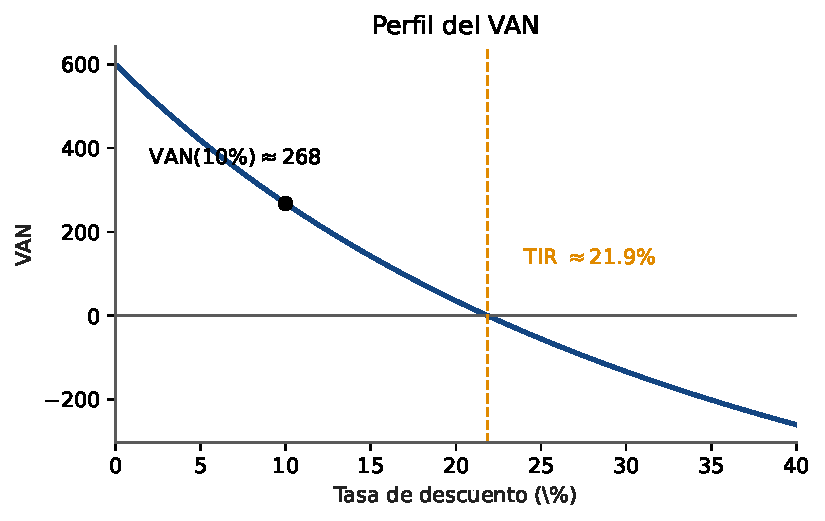
\includegraphics[width=0.72\linewidth]{figuras/van_perfil}
\caption{El perfil del VAN: a mayor tasa de descuento, menor VAN. La curva cruza el cero exactamente en la TIR, uniendo ambos criterios en una sola imagen.}
\label{fig:van_perfil}
\end{figure}

\section{La inversión, en el contexto macro}

¿De dónde sale la tasa de descuento? En buena medida, de las condiciones financieras de la economía. Blanchard~\cite{blanchard} subraya que la inversión agregada depende negativamente de la tasa de interés: tasas más altas encarecen el capital, suben la valla que un proyecto debe superar y, por lo tanto, hay menos proyectos con VAN positivo. Así, la decisión micro de una empresa (este capítulo) y la dinámica macro de la inversión (la macroeconomía) son dos miradas del mismo fenómeno \cite{blanchard}.

\begin{labbox}
La librería \texttt{numpy\_financial} implementa estos criterios directamente: \texttt{npv(tasa, flujos)} para el VAN, \texttt{irr(flujos)} para la TIR y \texttt{mirr(...)} para la TIRM. El payback descontado se calcula a mano, acumulando los flujos descontados hasta que el acumulado cruza cero. Y el perfil del VAN es, simplemente, evaluar \texttt{npv} para una lista de tasas y graficar: la curva corta el eje en la TIR, uniendo en una figura toda la teoría del capítulo.
\end{labbox}

\section{Síntesis del capítulo}

El valor tiempo del dinero obliga a descontar los flujos futuros. El VAN —crear o destruir valor— es el criterio rey; la TIR, el payback y la TIRM lo complementan desde la rentabilidad y la liquidez. Con esto cerramos el recorrido económico del curso: del precio de un bien a la decisión de invertir, todo el camino se apoya en las mismas funciones, derivadas, integrales y sistemas que vimos.

\chapter{Cierre: de la teoría al código}
\label{cap:cierre}

\section{Un mapa de todo lo recorrido}

Llegamos al final con una convicción que vale la pena hacer explícita: \textbf{los nueve bloques de este curso no son nueve temas sueltos, sino una sola historia}. Empezamos describiendo la actividad económica con funciones; las pusimos a interactuar para hallar equilibrios; medimos el cambio con derivadas y lo acumulamos con integrales; usamos ese cálculo para optimizar; llevamos la optimización al terreno estratégico del oligopolio; y proyectamos todo hacia el futuro con la evaluación de inversiones. Cada pieza se apoya en la anterior.

La siguiente tabla resume el puente entre cada concepto económico y la herramienta computacional que lo hace operativo en el laboratorio:

\begin{center}
\renewcommand{\arraystretch}{1.25}
\begin{tabular}{p{5.6cm} p{3.4cm} p{4.2cm}}
\toprule
\textbf{Concepto económico} & \textbf{Capítulo} & \textbf{Herramienta} \\
\midrule
Datos, variables y visualización & \ref{cap:datos} & \texttt{pandas}, \texttt{matplotlib} \\
Funciones (demanda, costo, ingreso) & \ref{cap:funciones} & \texttt{sympy}, \texttt{matplotlib} \\
Equilibrio de mercado & \ref{cap:equilibrio} & \texttt{sympy.solve} \\
Insumo-producto (Leontief) & \ref{cap:leontief} & \texttt{numpy.linalg} \\
Análisis marginal & \ref{cap:marginal} & \texttt{sympy.diff} \\
Elasticidad & \ref{cap:elasticidad} & \texttt{sympy}, \texttt{pandas} \\
Excedentes & \ref{cap:integrales} & \texttt{sympy.integrate} \\
Optimización & \ref{cap:optimizacion} & \texttt{sympy}, \texttt{PuLP} \\
Duopolio de Cournot & \ref{cap:duopolio} & \texttt{sympy.solve} (sistema) \\
Evaluación de inversiones & \ref{cap:inversiones} & \texttt{numpy\_financial} \\
\bottomrule
\end{tabular}
\end{center}

\section{Qué aporta cada mitad}

Conviene insistir en la división del trabajo entre el economista y la máquina, porque es el sentido último de la materia:

\begin{itemize}
  \item \textbf{La computadora} hace el cálculo: deriva, integra, invierte matrices, resuelve sistemas, descuenta flujos. Es rápida, exacta y no se cansa.
  \item \textbf{El economista} hace lo que la máquina no puede: \emph{plantear} el problema correcto, \emph{elegir} qué función representa la realidad, \emph{interpretar} si un resultado tiene sentido y \emph{decidir} en consecuencia.
\end{itemize}

Un VAN positivo no decide por vos; te informa. Una elasticidad de $-0.7$ no fija el precio; te dice que tenés margen para subirlo. El juicio económico —saber qué preguntar y cómo leer la respuesta— es insustituible, y es exactamente lo que esta materia busca entrenar.

\section{Para seguir}

Este material es una puerta de entrada, no una enciclopedia. Quien quiera profundizar encontrará en la microeconomía de \cite{varian}, \cite{pindyck} y \cite{nicholson}, en la matemática económica de \cite{chiang} y \cite{sydsaeter}, en las finanzas de \cite{brealey} y \cite{sapag}, y en la macro de \cite{blanchard}, desarrollos mucho más extensos de cada tema. Pero la lógica de fondo —traducir un problema de gestión a una estructura económica, resolverla con la herramienta adecuada e interpretar el resultado— es la que ya tenés, y la que vas a usar una y otra vez.

\begin{ideabox}
\textbf{La síntesis del curso, en una línea.} La teoría económica te dice \emph{qué} mirar; los métodos cuantitativos te dicen \emph{cuánto} vale; y el criterio profesional te dice \emph{qué hacer} con esa respuesta.
\end{ideabox}


\appendix
\chapter{Formulario}
\label{ap:formulario}

Resumen compacto de las fórmulas del curso, pensado como hoja de consulta rápida para parciales y trabajos prácticos. Cada bloque remite al capítulo donde se explica.

\section*{Funciones económicas (Cap.~\ref{cap:funciones})}
\begin{align*}
\text{Demanda / inversa:}\quad & Q_d = a - b\,p \;\Longleftrightarrow\; p = \tfrac{a}{b} - \tfrac{1}{b}Q \\
\text{Oferta:}\quad & Q_s = c + d\,p \\
\text{Costo total:}\quad & C(q) = CF + CV(q) \\
\text{Costo medio / marginal:}\quad & \cme = \tfrac{C(q)}{q}, \qquad \cmg = \tfrac{\dd C}{\dd q} \\
\text{Ingreso / Beneficio:}\quad & I(q) = p\cdot q, \qquad \Pi(q) = I(q) - C(q)
\end{align*}

\section*{Equilibrio de mercado (Cap.~\ref{cap:equilibrio})}
\[
Q_d = Q_s \;\Longrightarrow\; p^{*} = \frac{a-c}{b+d}, \qquad q^{*} = a - b\,p^{*}
\]

\section*{Insumo-producto de Leontief (Cap.~\ref{cap:leontief})}
\[
\mathbf{x} = A\mathbf{x} + \mathbf{d} \;\Longrightarrow\; \mathbf{x} = (I - A)^{-1}\,\mathbf{d}
\]
$a_{ij}=$ insumo de $i$ por unidad de $j$; \quad $(I-A)^{-1}=$ matriz de requerimientos totales.

\section*{Análisis marginal (Cap.~\ref{cap:marginal})}
\begin{align*}
f'(x) &= \lim_{h\to 0}\frac{f(x+h)-f(x)}{h}, \qquad
\tfrac{\dd}{\dd q}(q^n) = n\,q^{n-1} \\
\tfrac{\dd \cme}{\dd q} &= \tfrac{1}{q}\big(\cmg - \cme\big) \;\Rightarrow\; \cme \text{ mínimo cuando } \cmg = \cme
\end{align*}

\section*{Elasticidad (Cap.~\ref{cap:elasticidad})}
\[
\varepsilon = \frac{\dd Q}{\dd p}\cdot\frac{p}{Q}, \qquad
\img = p\Big(1 + \tfrac{1}{\varepsilon}\Big)
\]
$|\varepsilon|>1$ elástica (subir $p \Rightarrow I\downarrow$); \; $|\varepsilon|<1$ inelástica (subir $p \Rightarrow I\uparrow$); \; $|\varepsilon|=1$ ingreso máximo.

\section*{Integrales y excedentes (Cap.~\ref{cap:integrales})}
\begin{align*}
\int_a^b f(x)\dd x &= F(b)-F(a), \qquad C(q) = \int_0^q \cmg(u)\dd u + CF \\
EC &= \int_0^{q^{*}}\!\!\big(p_d(Q)-p^{*}\big)\dd Q, \qquad
EP = \int_0^{q^{*}}\!\!\big(p^{*}-p_s(Q)\big)\dd Q
\end{align*}

\section*{Optimización (Cap.~\ref{cap:optimizacion})}
\[
\text{CPO: } \Pi'(q^{*})=0 \Leftrightarrow \img=\cmg, \qquad
\text{CSO: } \Pi''(q^{*})<0
\]
Programación lineal: $\max\ \sum_j c_j x_j$ \ s.a. \ $\sum_j a_{ij}x_j \le b_i,\ x_j\ge 0$.

\section*{Duopolio de Cournot (Cap.~\ref{cap:duopolio})}
\[
q_1 = \frac{a - c - b\,q_2}{2b} \quad(\text{mejor respuesta}); \qquad
q^{*} = \frac{a-c}{3b}, \quad Q^{*} = \frac{2(a-c)}{3b}
\]

\section*{Evaluación de inversiones (Cap.~\ref{cap:inversiones})}
\begin{align*}
\van &= \sum_{t=0}^{n}\frac{F_t}{(1+r)^{t}} \quad(\text{aceptar si } \van>0) \\
\tir:\ & \sum_{t=0}^{n}\frac{F_t}{(1+\tir)^{t}} = 0 \quad(\text{aceptar si } \tir > r)
\end{align*}

\chapter{Glosario de términos}
\label{ap:glosario}

Definiciones breves de los conceptos centrales, para consulta rápida.

\begin{description}[style=nextline,leftmargin=0pt]
  \item[Beneficio ($\Pi$)] Diferencia entre el ingreso total y el costo total: $\Pi = I - C$.
  \item[Ceteris paribus] «Manteniendo todo lo demás constante». Supuesto para aislar el efecto de una sola variable.
  \item[Costo marginal ($\cmg$)] Costo de producir una unidad adicional; derivada del costo total.
  \item[Costo medio ($\cme$)] Costo total dividido por la cantidad: costo por unidad.
  \item[Demanda inversa] Función que da el precio en función de la cantidad, $p(Q)$; despeje de la demanda.
  \item[Elasticidad ($\varepsilon$)] Variación porcentual de una variable ante la variación porcentual de otra; medida adimensional de sensibilidad.
  \item[Equilibrio de mercado] Precio y cantidad donde la cantidad demandada iguala a la ofrecida.
  \item[Equilibrio de Nash] Situación en que ninguna parte gana desviándose, dadas las decisiones de las demás.
  \item[Estática comparativa] Comparación de dos equilibrios antes y después de cambiar un parámetro.
  \item[Excedente del consumidor (EC)] Diferencia entre lo que los consumidores estaban dispuestos a pagar y lo que pagaron.
  \item[Excedente del productor (EP)] Diferencia entre el precio recibido y el costo marginal de cada unidad.
  \item[Ingreso marginal ($\img$)] Ingreso adicional por vender una unidad más; derivada del ingreso total.
  \item[Matriz de Leontief] $(I-A)^{-1}$: requerimientos totales (directos e indirectos) de producción por unidad de demanda final.
  \item[Mediana] Valor que deja la mitad de los datos por debajo y la mitad por encima; medida robusta.
  \item[Optimización] Búsqueda del valor de una variable que maximiza o minimiza una función objetivo.
  \item[Payback (período de recupero)] Tiempo necesario para recuperar la inversión inicial con los flujos del proyecto.
  \item[Programación lineal] Optimización de un objetivo lineal sujeto a restricciones lineales.
  \item[TIR] Tasa de descuento que hace el VAN igual a cero; rentabilidad propia del proyecto.
  \item[Valor tiempo del dinero] Principio de que un peso hoy vale más que un peso en el futuro.
  \item[VAN] Valor Actual Neto: suma de los flujos de un proyecto descontados al presente.
\end{description}


% ============================================================
%  BIBLIOGRAFÍA
% ============================================================
\begin{thebibliography}{99}
\addcontentsline{toc}{chapter}{Bibliografía}

\bibitem[Blanchard et al. (2017)]{blanchard}
Blanchard, O., Amighini, A. y Giavazzi, F. (2017). \textit{Macroeconomía} (7.\textsuperscript{a} ed.). Pearson.

\bibitem[Brealey et al. (2020)]{brealey}
Brealey, R., Myers, S. y Allen, F. (2020). \textit{Principios de finanzas corporativas} (13.\textsuperscript{a} ed.). McGraw-Hill.

\bibitem[Chiang y Wainwright (2006)]{chiang}
Chiang, A. y Wainwright, K. (2006). \textit{Métodos fundamentales de economía matemática} (4.\textsuperscript{a} ed.). McGraw-Hill.

\bibitem[Gibbons (1992)]{gibbons}
Gibbons, R. (1992). \textit{Un primer curso de teoría de juegos}. Antoni Bosch.

\bibitem[Leontief (1986)]{leontief}
Leontief, W. (1986). \textit{Input-Output Economics} (2.\textsuperscript{a} ed.). Oxford University Press.

\bibitem[Mankiw (2020)]{mankiw}
Mankiw, N. G. (2020). \textit{Principios de economía} (8.\textsuperscript{a} ed.). Cengage.

\bibitem[Nicholson y Snyder (2017)]{nicholson}
Nicholson, W. y Snyder, C. (2017). \textit{Teoría microeconómica: principios básicos y ampliaciones} (11.\textsuperscript{a} ed.). Cengage.

\bibitem[Pindyck y Rubinfeld (2018)]{pindyck}
Pindyck, R. y Rubinfeld, D. (2018). \textit{Microeconomía} (9.\textsuperscript{a} ed.). Pearson.

\bibitem[Sapag Chain (2011)]{sapag}
Sapag Chain, N. (2011). \textit{Proyectos de inversión: formulación y evaluación} (2.\textsuperscript{a} ed.). Pearson.

\bibitem[Stiglitz y Walsh (2009)]{stiglitz}
Stiglitz, J. y Walsh, C. (2009). \textit{Microeconomía} (4.\textsuperscript{a} ed.). Ariel.

\bibitem[Sydsæter y Hammond (2012)]{sydsaeter}
Sydsæter, K. y Hammond, P. (2012). \textit{Matemáticas para el análisis económico}. Prentice Hall.

\bibitem[Varian (2010)]{varian}
Varian, H. (2010). \textit{Microeconomía intermedia: un enfoque actual} (8.\textsuperscript{a} ed.). Antoni Bosch.

\end{thebibliography}

\end{document}
